% couette-flow-3D.tex

\newpage
\section{Couette Flow: 3D}
\label{couette-flow-3D}\index{boundary conditions!MovingWallBC!example of use}
%
This three-dimensional Couette flow case is provided by Jason Qin, 
as an extension of the two-dimensional case in Sec\,\ref{couette-flow-2D}.
The front and side views of the flow doamin are shown in Figure~\ref{couette3-frontside-fig}. 
Since we are going to monitor the velocity profile between the plates 
that are separated by a small distance in $z$ direction, 
the grid has high resolution in that direction compared 
to the resolutions in $x$ and $y$ directions. 

\begin{figure}[htbp]
\begin{center}
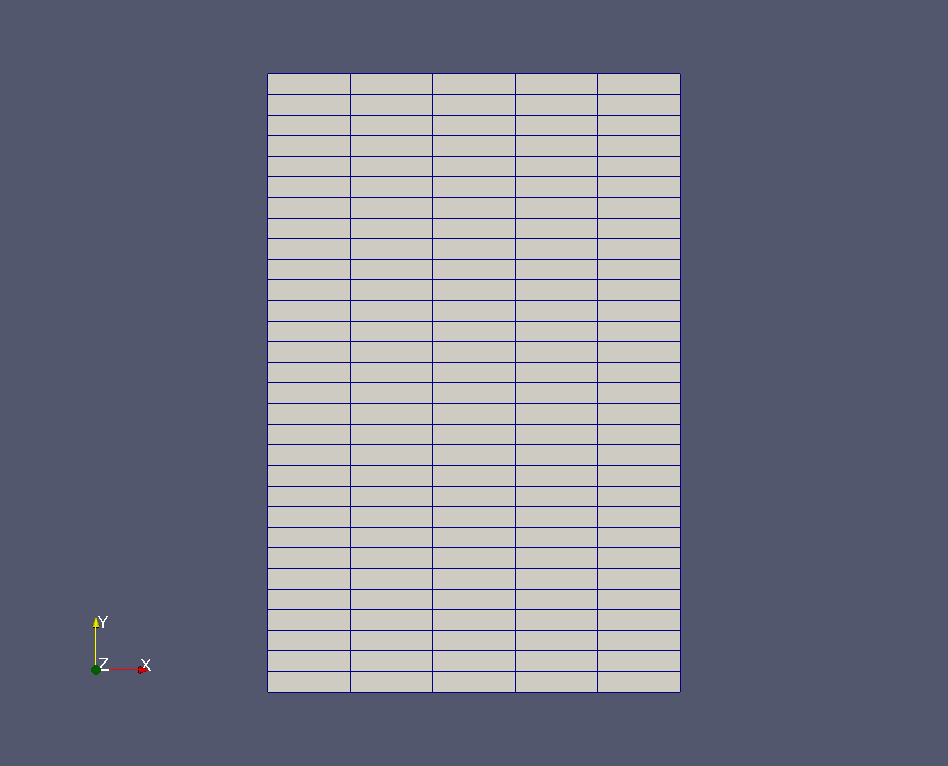
\includegraphics[width=0.45\textwidth]{../3D/couette-flow/front-view.png}
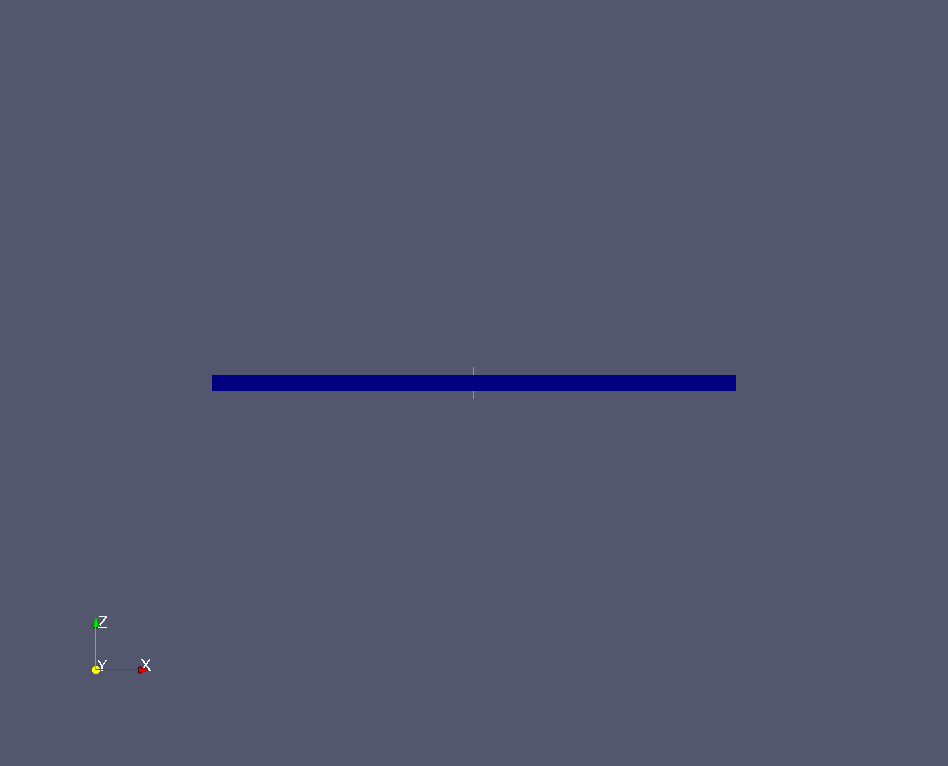
\includegraphics[width=0.45\textwidth]{../3D/couette-flow/side-view.png}
\end{center}
\caption{Front and side view of 3D couette flow.}
   \label{couette3-frontside-fig}
\end{figure}

\bigskip
\subsection{Input script (.py)}
%
The top surface is set as Moving-Wall boundary condition, while the BOTTOM surface Adiabatic-Wall.
These are effectively the two plates that bound the flow.
Slip-Wall boundary conditions were set both the the WEST and EAST surface, 
while the NORTH and SOUTH surfaces are connected manually
with the aid of the function \verb!connect_blocks_3D!.
Since the NORTH and SOUTH boundary surfaces are not geometrically adjacent, 
the boolean parameter of \verb!check_corner_locations! should be
set to \verb!False!, else the \verb!connect_blocks_3D! will flag an error.

\noindent\topbar
\lstinputlisting[language={}]{../3D/couette-flow/couette.py}
\bottombar


\subsection{Shell scripts}
\label{couette-flow-3D-sh-files}
\topbar
\lstinputlisting[language={}]{../2D/couette-flow/couette.sh}
\bottombar

\subsection{Results}
%
The velocity profile along the height with different initial values are 
shown in Figure~\ref{couette3-linearuniform-fig}, respectively. 
The form of the initial velocity profile has a big effect on the computation time for this test case, 
with the uniform velocity requiring a long simulation time to reach steady state, 
compared with a linear initial velocity profile.

\begin{figure}[htbp]
\begin{center}
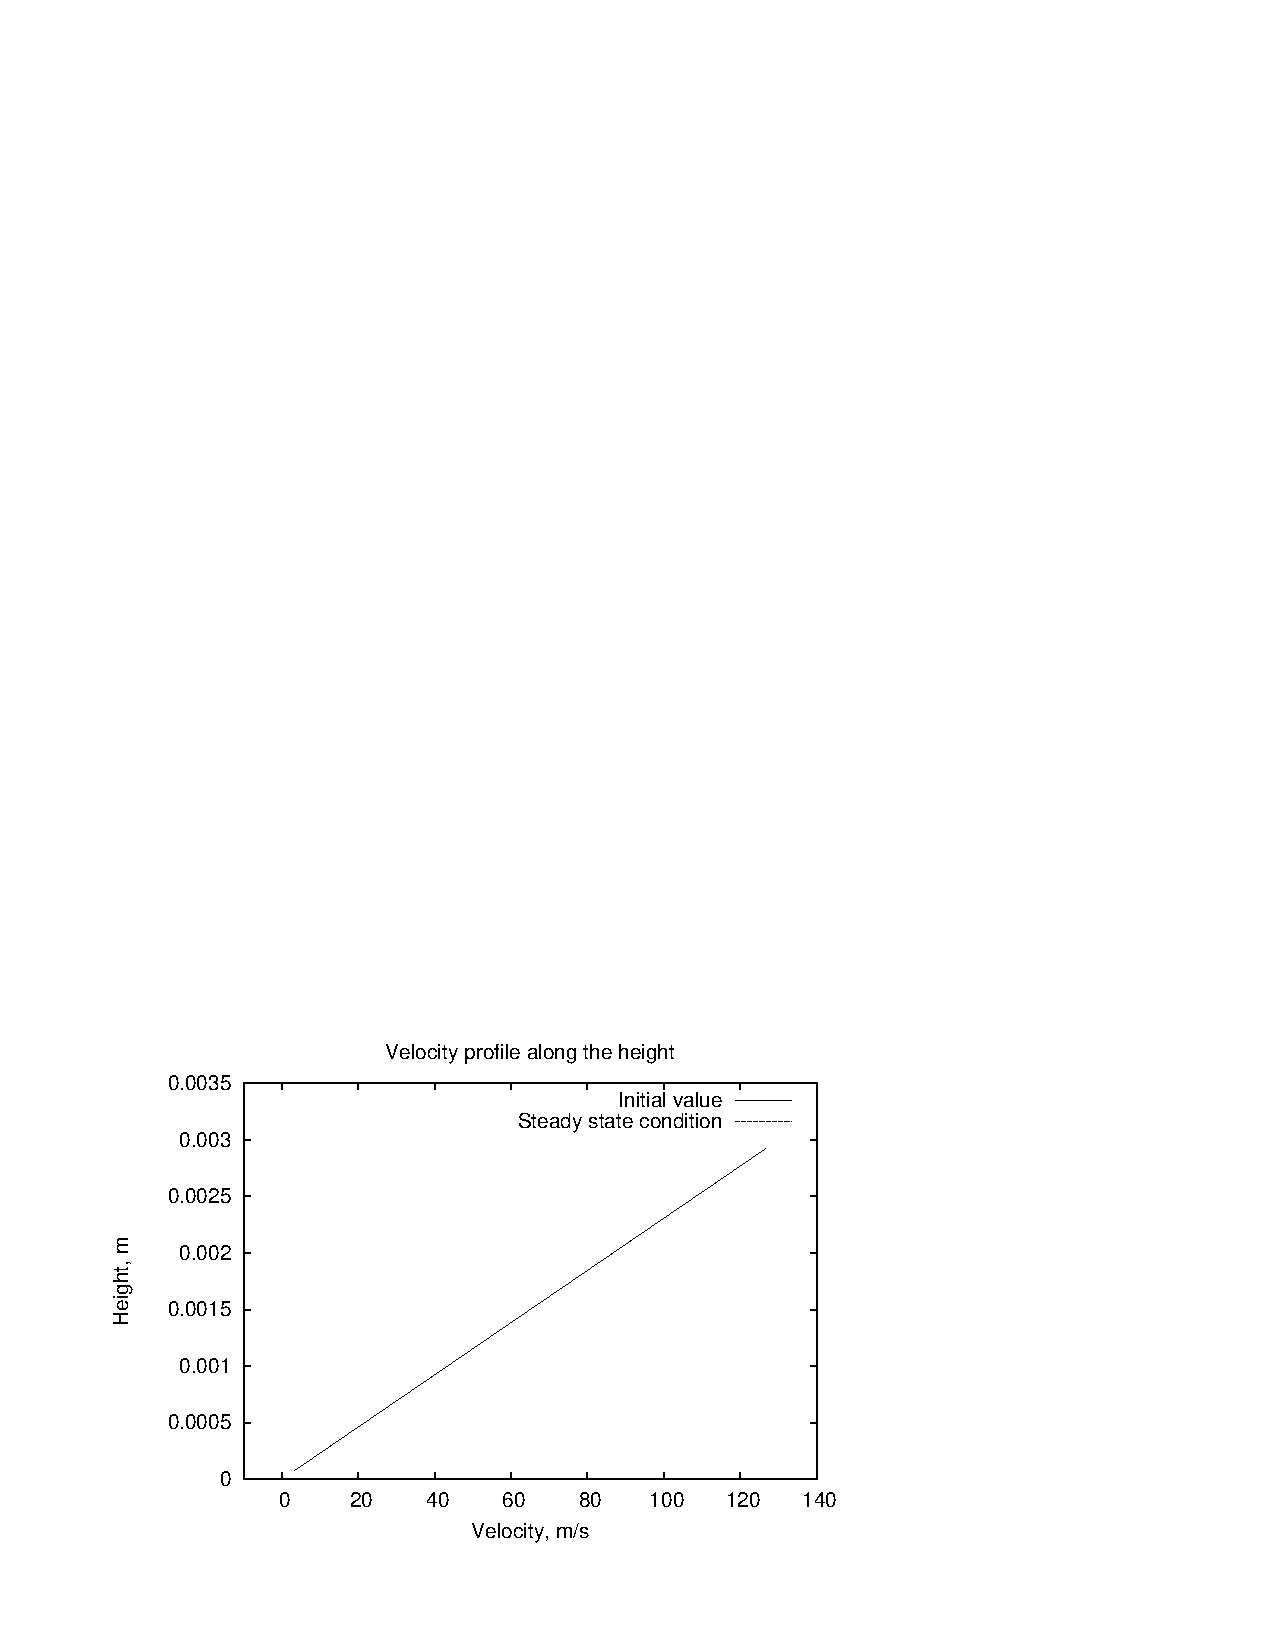
\includegraphics[width=0.45\textwidth,viewport=39 52 414 298,clip=true]{../3D/couette-flow/c_3D_linear.pdf}
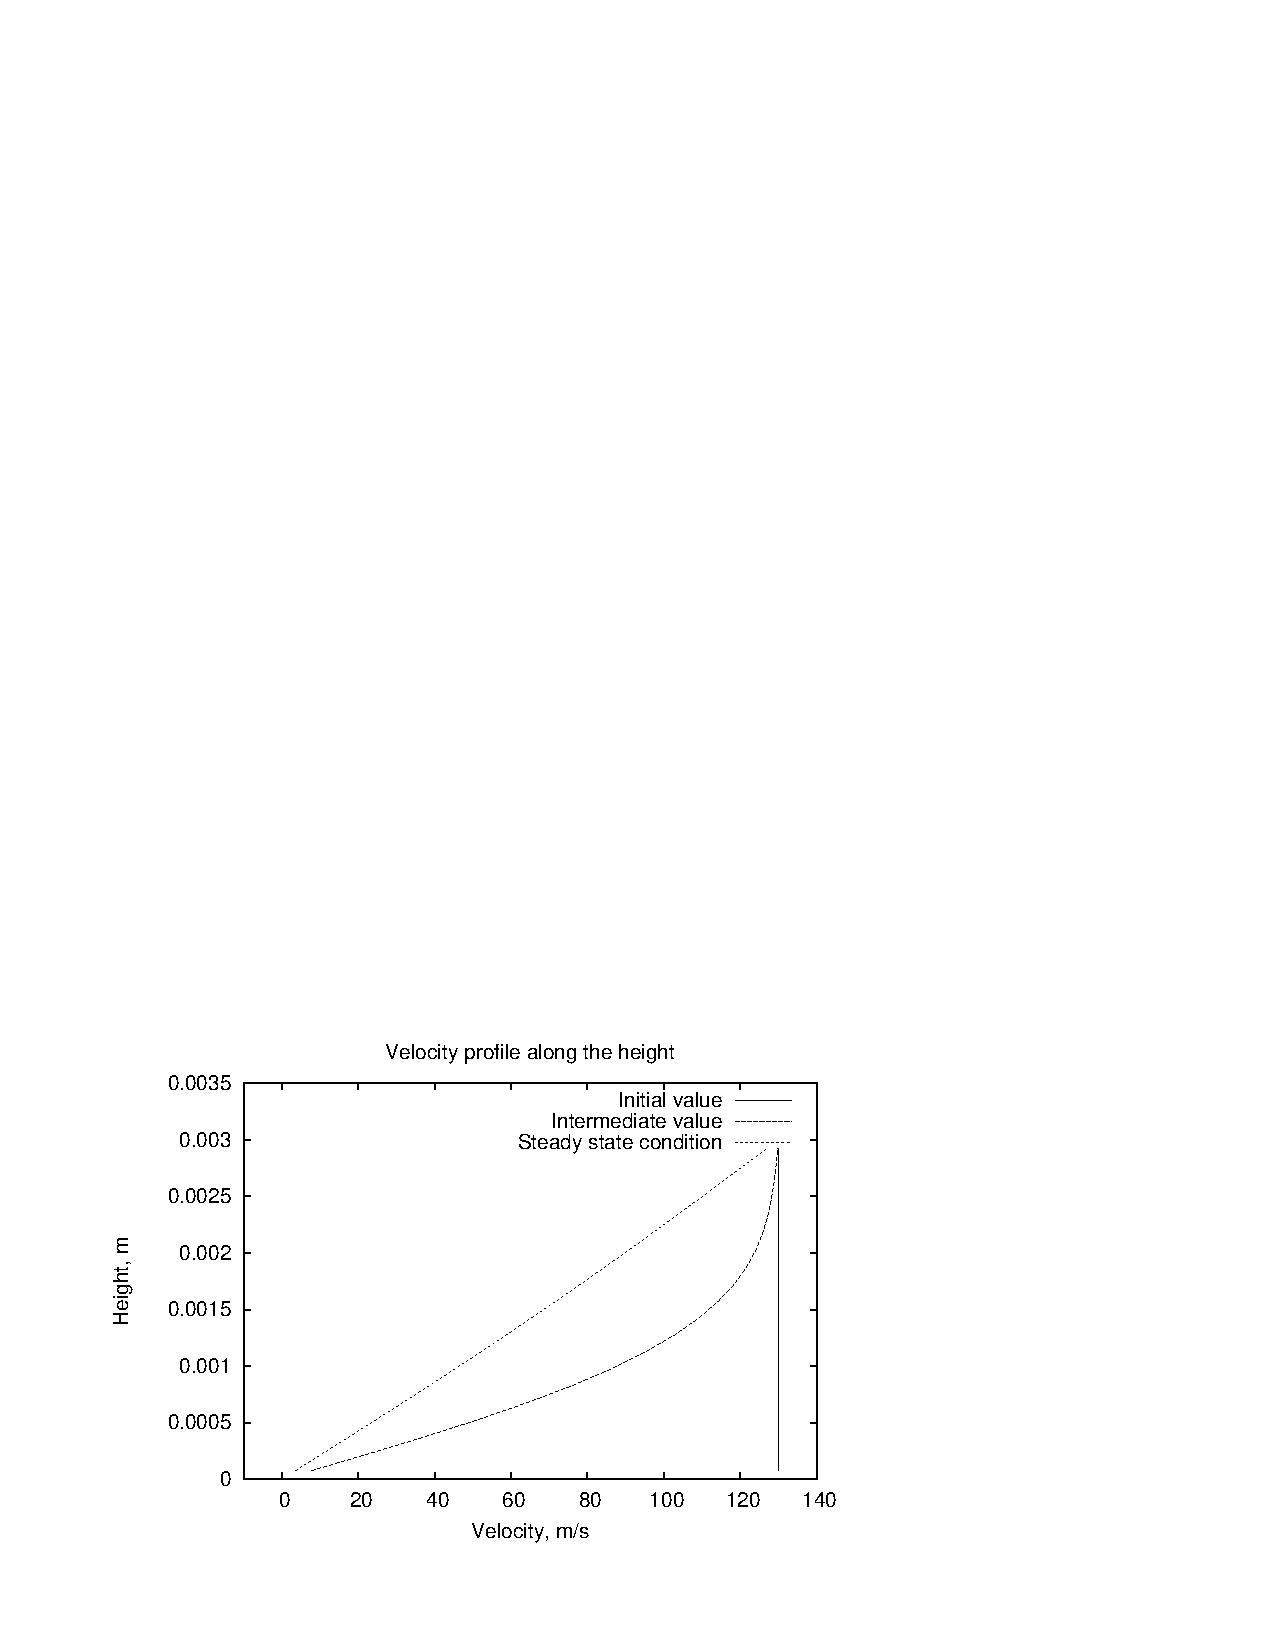
\includegraphics[width=0.45\textwidth,viewport=39 52 414 298,clip=true]{../3D/couette-flow/c_3D_uniform.pdf}
\end{center}
\caption{Velocity profile along the height: linear and uniform initial velocity profiles.}
   \label{couette3-linearuniform-fig}
\end{figure}


\subsection{Notes}
\begin{itemize}
\item None
\end{itemize}


